\documentclass[a4paper,12pt]{article}
\usepackage[utf8]{inputenc}
\usepackage[ngerman]{babel}
\usepackage{amsmath, amssymb}
\usepackage{graphicx}
\usepackage{float}
\usepackage{geometry}
\usepackage{booktabs}
\geometry{a4paper, margin=1in}

\title{Bestimmung der Fluchtgeschwindigkeit und der Hubble-Konstanten}
\author{Astronomisches Praktikum \\
Sommersemester 2024\\\\
Guilherme Schmid}
\date{}

\begin{document}

\maketitle

\section*{Zielsetzung}
Ziel des Versuches war es, die Spektren von Galaxien zu analysieren, um deren Fluchtgeschwindigkeiten und Entfernungen zu bestimmen. Darüber hinaus sollte die Hubble-Konstante ermittelt und das Weltalter sowie der Weltradius abgeschätzt werden.

\section*{Durchführung}
Die Untersuchung basiert auf den Ca II H\&K-Absorptionslinien in den Galaxienspektren und den Vergleichsspektren der He I-Lampe. Die folgenden Schritte wurden durchgeführt:
\begin{enumerate}
	\item \textbf{Messung der Abstände}: Die Abstände der H\&K-Linien zu den He I-Linien wurden in Millimetern gemessen.
	\item \textbf{Berechnung der Dispersion}: Die Dispersion des Spektrums in Å/mm wurde berechnet, um die gemessenen Abstände in Wellenlängen umzurechnen.
	\item \textbf{Bestimmung der Fluchtgeschwindigkeit}: Mit den umgerechneten Wellenlängen und den Ruhewellenlängen wurden die Fluchtgeschwindigkeiten berechnet.
	\item \textbf{Berechnung der Entfernungen}: Die Entfernungen zu den Galaxien wurden aus den gemessenen Winkeldurchmessern und einem angenommenen tatsächlichen Durchmesser berechnet.
	\item \textbf{Hubble-Diagramm}: Die berechneten Fluchtgeschwindigkeiten und Entfernungen wurden in einem Hubble-Diagramm dargestellt, um die Hubble-Konstante zu bestimmen.

\end{enumerate}

\section*{Auswertung}
\begin{table}[H]
    \centering
    \begin{tabular}{cccc}
        \toprule
        Galaxie & Abstand K (mm) & Abstand H (mm) & Fluchtgeschwindigkeit (km/s) \\
        \midrule
        Virgo & 4 & 5 & 6085.47 \\
        Ursa Major & 14 & 17 & 20962.37 \\
        Corona Borealis & 21 & 24 & 30433.29 \\
        Bootes & 33 & 36 & 46669.14 \\
        Hydra & 51 & 53 & 70349.41 \\
        \bottomrule
    \end{tabular}
    \caption{Abstände der Ca II H\&K-Linien und berechnete Fluchtgeschwindigkeiten.}
    \label{tab:fluchtgeschwindigkeit}
\end{table}

\subsection*{Berechnung der Dispersion}
Die Dispersion wurde mittels der gemessenen Abstände der He I-Linien zur Linie a berechnet:
\begin{align*}
\text{Dispersion (b - a)} &= 19.00 \, \text{Å/mm} \\
\text{Dispersion (c - a)} &= 19.643 \, \text{Å/mm} \\
\text{Dispersion (d - a)} &= 18.221 \, \text{Å/mm} \\
\text{Dispersion (e - a)} &= 16.651 \, \text{Å/mm} \\
\text{Dispersion (f - a)} &= 16.824 \, \text{Å/mm} \\
\text{Dispersion (g - a)} &= 16.574 \, \text{Å/mm} \\
\text{Mittlere Dispersion} &= 17.819 \, \text{Å/mm}
\end{align*}

\subsection*{Berechnung der Fluchtgeschwindigkeit}
Die beobachteten Wellenlängen der H\&K-Linien wurden mit der mittleren Dispersion umgerechnet. Die Fluchtgeschwindigkeiten wurden nach Gleichung (5.2) berechnet.

\subsection*{Entfernungen der Galaxien}
Die Entfernungen der Galaxien wurden aus den gemessenen Winkeldurchmessern und dem angenommenen tatsächlichen Durchmesser von $s = 0.02 \, \text{Mpc}$ berechnet.

\begin{table}[H]
    \centering
    \begin{tabular}{cc}
        \toprule
        Galaxie & Entfernung $d$ (Mpc) \\
        \midrule
        Virgo & 31.84 \\
        Ursa Major & 121.01 \\
        Corona Borealis & 201.68 \\
        Bootes & 605.04 \\
        Hydra & 605.04 \\
        \bottomrule
    \end{tabular}
    \caption{Entfernungen der Galaxien.}
    \label{tab:entfernungen}
\end{table}

\begin{figure}[H]
    \centering
    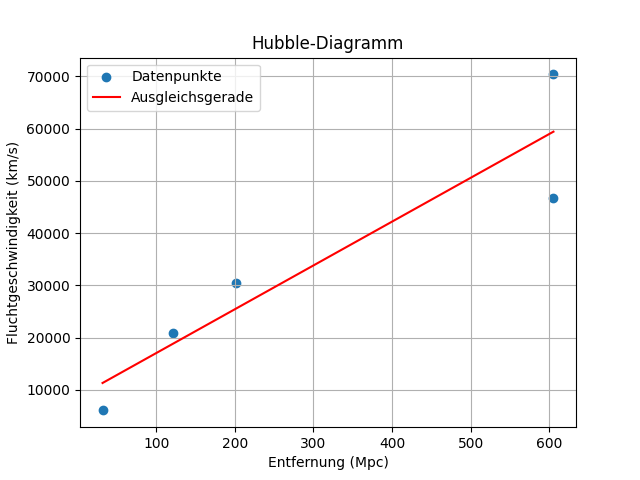
\includegraphics[width=0.8\textwidth]{HubbleDiagramm.png}
    \caption{Hubble-Diagramm der berechneten Entfernungen und Fluchtgeschwindigkeiten.}
    \label{fig:hubble_diagramm}
\end{figure}

\section*{Fazit}
Die Hubble-Konstante wurde aus der Steigung der Ausgleichsgeraden im Hubble-Diagramm berechnet:
\begin{align*}
H &= 83.86 \, \text{km/s/Mpc}
\end{align*}

\subsection*{Weltalter und Weltradius}
Das Weltalter $T$ und der Weltradius $D$ wurden nach den Gleichungen (5.3) und (5.4) bestimmt:
\begin{align*}
T &= \frac{1}{H} = 0.0119 \, \text{Gyr} \\
D &= \frac{c}{H} = 3577.35 \, \text{Mpc}
\end{align*}

\section*{Anhang}
Die Berechnungen wurden mit Hilfe eines Python-Skripts durchgeführt, welches die erforderlichen Messdaten und Berechnungen automatisiert hat.

\end{document}